\documentclass{article}

% if you need to pass options to natbib, use, e.g.:
% \PassOptionsToPackage{numbers, compress}{natbib}
% before loading nips_2017
%
% to avoid loading the natbib package, add option nonatbib:
% \usepackage[nonatbib]{nips_2017}

%\usepackage{main}

% to compile a camera-ready version, add the [final] option, e.g.:
\usepackage[final]{main}

\usepackage[utf8]{inputenc} % allow utf-8 input
\usepackage[T1]{fontenc}    % use 8-bit T1 fonts
\usepackage{hyperref}       % hyperlinks
\usepackage{url}            % simple URL typesetting
\usepackage{booktabs}       % professional-quality tables
\usepackage{amsfonts}       % blackboard math symbols
\usepackage{nicefrac}       % compact symbols for 1/2, etc.
\usepackage{microtype}      % microtypography
\usepackage{multicol}
\usepackage{graphicx}
\usepackage{amsmath}
\usepackage{bbm}
\usepackage{enumerate}
\usepackage[linguistics]{forest}
\usepackage{adjustbox}
\usepackage{bbm}
\usepackage{amssymb}
\usepackage{mathtools}
\DeclarePairedDelimiter{\ceil}{\lceil}{\rceil}
\DeclarePairedDelimiter{\floor}{\lfoor}{\rfloor}
%\usepackage[margin=0.5in]{geometry}
%\DeclareMathOperator*{\argmax}{argmax}

\usepackage{listings}
\usepackage{color}
 
\definecolor{codegreen}{rgb}{0,0.6,0}
\definecolor{codegray}{rgb}{0.5,0.5,0.5}
\definecolor{codepurple}{rgb}{0.58,0,0.82}
\definecolor{backcolour}{rgb}{0.95,0.95,0.92}
 
\lstdefinestyle{mystyle}{
    backgroundcolor=\color{backcolour},   
    commentstyle=\color{codegreen},
    keywordstyle=\color{magenta},
    numberstyle=\ttfamily\tiny\color{codegray},
    stringstyle=\color{codepurple},
    basicstyle=\ttfamily\small,
    columns=fullflexible,
    breakatwhitespace=false,         
    breaklines=true,                 
    captionpos=t,                    
    keepspaces=true,                 
    numbers=left,                    
    numbersep=5pt,                  
    showspaces=false,                
    showstringspaces=false,
    showtabs=false,                  
    tabsize=4,
}
 
\lstset{style=mystyle}

\title{Graphics Processing Units - Fall 2018\\
       \Large Homework 2}
\graphicspath{{images/}}
\setcitestyle{round, sort, numbers}

% The \author macro works with any number of authors. There are two
% commands used to separate the names and addresses of multiple
% authors: \And and \AND.
%
% Using \And between authors leaves it to LaTeX to determine where to
% break the lines. Using \AND forces a line break at that point. So,
% if LaTeX puts 3 of 4 authors names on the first line, and the last
% on the second line, try using \AND instead of \And before the third
% author name.

\author{
  Daniel Rivera Ruiz\\
  Department of Computer Science\\
  New York University\\
  \href{mailto:drr342@nyu.edu}{\texttt{drr342@nyu.edu}}\\
}

\begin{document}

\maketitle

% \cite{} - in-line citation author, year in parenthesis.
% \citep{} - all citation info in parenthesis.

%	\begin{figure}[ht]
%		\centering
%		\frame{
%            \includegraphics[width=1.0\linewidth]{tree.png}
%       }
%		\caption{Classification results for the sentence \textit{"There are slow and repetitive parts, but it has just enough spice to keep it                  interesting."} using the Stanford Sentiment Treebank. As can be seen, sentiment scores are available for each phrase.}
%		\label{tree}
%	\end{figure}

\begin{enumerate}[1.]
    \item Assume the following piece of code is running on G80:
	\begin{figure}[ht]
		\centering
            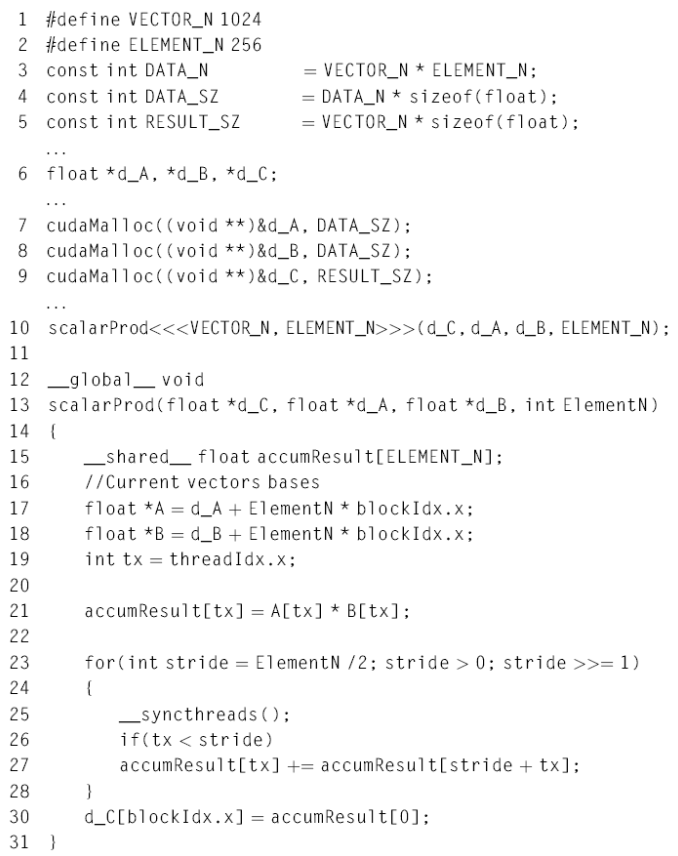
\includegraphics[width=0.75\linewidth]{Code.PNG}
		\label{code}
	\end{figure}
	\begin{enumerate}[(a)]
	    \item How many threads are there in total?\\
	    There are \texttt{ELEMENT\_N}$=256$ threads per block and there are \texttt{VECTOR\_N}$=1\,024$ blocks, so the total number of threads is $1\,024 \cdot 256 = \mathbf{262\,144}$.
	    \item How many threads are there in a warp?\\
	    The number of threads per warp is fixed for all Nvidia GPUs and it is equal to $\mathbf{32}$.
	    \item How many threads are there in a block?\\
	    As stated in (a), the number of threads per block is $\mathbf{256}$.
	    \item How many global memory loads and stores are done for each thread?\\
	    According to the \emph{CUDA C Programming Guide}, \texttt{\_\_global\_\_} function parameters are passed to the device via constant memory, which means that lines 17, 18 and 19 are only accessing either constant memory or registers. Therefore, per thread there are only two load operations (on line 21, one for \texttt{A[tx]} and one for \texttt{B[tx]}) and one store operation (on line 30 for \texttt{d\_C[blockIdx.x]}).
	    \item How many accesses to shared memory are done for each block?
	    \begin{itemize}
	        \item On line 21 there is one write operation to shared memory (\texttt{accumResult[tx]}) per thread, so $\mathbf{256}$ in total.
	        \item Within the \texttt{for} loop, line 27 is executed by half of the threads on the first iteration. For further iterations the number of threads that execute the line is halved. Each execution of this line requires two accesses to shared memory (one read of \texttt{accumResult[stride+tx]} and one write to \texttt{accumResult[tx]}). Therefore, the total number of accesses associated to the \texttt{for} loop is $2\cdot(128+64+32+16+8+4+2+1) = \mathbf{510}$.
	        \item Finally, on line 30 each thread reads \texttt{accumResult[0]}, which results in $\mathbf{256}$ accesses.
	        \item The total number of accesses to shared memory per block is therefore $256 + 510 + 256 = \mathbf{1\,022}$.
	    \end{itemize}
	    \item How many iterations of the for loop (Line 23) will have branch divergence? Show your derivation.\\
	    Branch divergence is calculated per warp, and the condition for divergence is introduced by line 26: \texttt{if (tx < stride)}. Therefore, as long as \texttt{(stride \% WARP\_SIZE) = 0} there will not be divergence within the warp. In the previous exercise we noticed that $\text{stride}(i) = 2^{7-i}, i \in [0,7]$, and since we know that \texttt{WARP\_SIZE = 32}, it is clear that the first 3 iterations ($\text{stride} = \{128, 64, 32\}$) won't have divergence and the last 4 ($\text{stride} = \{16, 8, 4, 2, 1\}$) will.
	    \item Identify an opportunity to significantly reduce the bandwidth requirement on
        the global memory. How would you achieve this? How many accesses can you eliminate?\\
        The accesses to global memory on line 21 are already optimized and cannot be avoided: 
        \begin{itemize}
            \item Each thread is reading one element from $A$ and one from $B$.
            \item There's no point on storing these values in shared memory because they will only be used once.
            \item Consecutive threads read consecutive addresses in memory, so the memory access is coalesced.
        \end{itemize}
        On line 30, however, the writing to global memory is very inefficient because all threads within the block are writing the same value (\texttt{accumResult[0]}) to the same location in global memory (\texttt{d\_C[blockIdx.x]}), effectively overwriting it $256$ times. To avoid this, line 30 can be replaced with the following:
\begin{lstlisting}[language=C]
if (tx < WARP_SIZE) {
    d_C[blockIdx.x] = accumResult[0];
}\end{lstlisting}
        By doing this small change, we reduce the number of writes to global memory per block from $256$ to $32$, while avoiding branch divergence within the warps of the block.
	\end{enumerate}
	
	\item What factors can make two threads corresponding to two different warps but of the same block take different amounts of time to finish? To get full credit, write at least 3 factors.
	\begin{itemize}
	    \item \emph{Conditional statements}. Even though branch divergence (within a warp) can be avoided by a well designed condition, different execution times for different warps will be almost inevitable, unless the instructions within both branches of the condition take similar amounts of time to execute.
	    \item \emph{Memory access}. If the memory being accessed by one of the threads is relevant to the whole application, it is more likely to be cached. Under this circumstances, the execution of this thread will be considerably faster compared to a thread that has to constantly fetch data from global memory.
	    \item \emph{Hardware considerations} It might be the case that the hardware associated to a given thread (SP) is inherently slower due to small variations in the manufacturing process of the device that cannot be avoided nor predicted.
	\end{itemize}
	
	\item What is the difference between shared memory and L1 cache?\\
	While both memories share the same on-chip physical location that considerably reduces latency compared to global memory access, the main difference between shared memory and L1 cache is the level of flexibility that they offer to the programmer.\\
	In the case of L1 cache this flexibility very limited, since the caching policies are unknown and hard to predict. Additionally, one line of the L1 cache is usually 128 bytes, so if the memory access of the application is not coalesced to make the most out of the line, cache misses will become more frequent.\\
	In contrast, the programmer has full control over the contents of shared memory and he makes it explicit within his code. This means that he can bring data from global memory into shared memory at will (as long as it fits) and at any level of granularity (non-coalesced access is possible, although discouraged if performance is to be maximized). Since shared memory is available to all the threads within a block, it facilitates and speeds up communication and data transfer among them, making it a very powerful resource when used properly.
	
	\item Can memory be coalesced for threads in a warp yet not-coalesced for threads in a different warp of the same block?\\
	It is possible. The following portion of code shows an example of this:
\begin{lstlisting}[language=C]
__global__ void kernel(float * A, float * B, int n) {
    if (threadIdx.x < WARP_SIZE) {
        B[threadIdx.x] = A[threadIdx.x];
    } else {
        B[threadIdx.x] = A[n * threadIdx.x];
    }
}\end{lstlisting}
    This kind of behaviour might not be very useful nor desired in most circumstances, but it is a simple instance where threads within the first warp of the block ($0 \leq \texttt{threadIdx.x} < 32$) will have coalesced memory access, and all other threads will not (assuming that $n \neq 1$).
	
	\item Suppose you want to write a kernel that operates on an image of size $(400 \times 900)$
    pixels. You want to assign one thread to each pixel. Your thread blocks are square
    in geometry, and you try to use the maximum number of threads per block possible on
    the device. The maximum number of threads per block is 1024. How would you
    select the grid dimensions and block dimensions of your kernel?\\
    Let $N$ be the size of the squared blocks $B = (N \times N)$, and let $W = \lceil\frac{400}{N}\rceil$ and $H = \lceil\frac{900}{N}\rceil$ be the dimension of the grid $G = (W \times H)$. The number of unused threads $U$ at the device level is given by the following expression:
    \begin{equation*}
        U = \left(WHN^2 - 400\cdot900\right) + \left(WH(-N^2 \text{ mod }32)\right) \\
    \end{equation*}
    Where the first part accounts for the threads that will be unused if the blocks don't fit exactly the size of the input grid, and the second part accounts for the threads within each block that will be unused if the number of threads per block is not a multiple of the warp size ($32$).\\
    So the problem is reduced to finding the value of $N$ that minimizes $U$:
    \begin{equation*}
        N^* = \underset{1 \leq N \leq 32}{argmin}(U)
    \end{equation*}
    If we simply tabulate for all possible values of $N$, we find that $N=8$ yields the optimal solution with $U=1\,600$, $W=50$ and $H=113$.\\
    This result shows that as a rule of thumb it is better to optimize for the number of threads within a block to be a multiple of the warp size, even if that means generating some extra threads in the grid. This makes sense because at least there is a guarantee that each block will fully span a certain number of warps.\\
    Trying to optimize for the blocks to fit exactly the dimensions of the input data is much more risky: at first glance it will look as if there were no unused threads within the grid, but under the hood as many as 31 threads can be idle each time the warp scheduler schedules the last warp of a block.
    % \begin{itemize}
    %     \item Select the block dimension $N$ in such a way that the blocks fit perfectly in the grid of pixels $(400 \times 900)$. Doing this there are no unused threads at the grid level, but there are $\frac{400\cdot900\cdot}{N^2}(N^2 (\text{mod}32))$ in total. 
    % \end{itemize}
    % The grid dimensions would be $\mathbf{G=(50 \times 113)}$, and the block dimensions would be $\mathbf{B=(8 \times 8)}$.
    % \begin{itemize}
    %     \item First we find the possible values for the size of the block $N$. Since $N^2$ can be at most $1\,024$ and at least $32$ (in order to use all the threads within a warp) we write 
    %     \begin{align*}
    %         32 \leq &N^2 \leq 1\,024\\
    %         \sqrt{32} \leq &N \leq 32\\
    %         &N \in \{8, 16, 64\}
    %     \end{align*}
    %     \item Once we have the size of the block, we can calculate the minimum number of blocks required to cover all the pixels. If $W$ and $H$ are the width and height of the grid:
    %     \begin{align*}
    %         WN &\geq 400 \\
    %         W &= \left\lceil\frac{400}{N}\right\rceil = \left\lceil\frac{400}{32}\right\rceil = 13 \\
    %         HN &\geq 900 \\
    %         H &= \left\lceil\frac{900}{N}\right\rceil = \left\lceil\frac{900}{32}\right\rceil = 29 \\     
    %     \end{align*}
    % \end{itemize}
    % This solution generates $13\cdot29\cdot32\cdot32=386\,048$ threads
    
    \item Suppose an NVIDIA GPU has 8 SMs. Each SM has 32 SPs, but a single warp is only 16
    threads. The GPU is to be used to add two arrays element-wise. Assume that the number of array
    elements is $2^{24}$. Let $t$ denote the amount of time it takes one thread (yes, just one) to perform the
    entire calculation on the GPU. The kernel code is shown below (\texttt{num\_threads} is the total number
    of threads in the whole GPU):
\begin{lstlisting}[language=C]
__device__ void prob(int array_size) {
    int tid = threadIdx.x + blockIdx.x * blockDim.x;
    for ( int i=tid; i<array_size; i += num_threads )
        result[i] = a[i] + b[i];
}\end{lstlisting}
    \begin{enumerate}[(a)]
        \item What is the amount of time it takes if we use one block of 16 threads?\\
        Since the block will fill entirely one warp it can be scheduled all at once. The 16 threads will run in parallel and effectively take the same amount of time $t$ of a single thread (though the cumulative time for all threads will obviously be $16t$). Since there are $2^{24}$ elements to process and each block processes 16 elements at a time, we need $2^{24} / 16 = 2^{20}$ blocks to perform the whole calculation. Each SM can handle 2 blocks (since it has twice the SPs as the size of the warp) and we have 8 SMs, so we can execute $8 \cdot 2 = 16$ blocks at once in the whole GPU. The overall running time for the whole application will therefore be:
        \begin{equation*}
            T_a = \frac{2^{20}t}{16} = 2^{16}t
        \end{equation*}
        \item What is the amount of time it takes if we use two blocks of 8 threads each?\\
        In this case each block is wasting half the threads in a warp, because one warp is the smallest scheduling unit and warps cannot span multiple blocks. All other things being the same, we know that the overall running time of the application will be:
        \begin{equation*}
            T_b = \frac{2^{21}t}{16} = 2^{17}t = 2 T_a
        \end{equation*}
        \item Justify why the above two answers are similar/different.\\
        As explained in the previous answer, half the threads in the whole device are being wasted because the size of the block is too small. Thus, the time required with blocks of size 8 is double the time required with blocks of size 16.
        \item Assume that 256 threads are enough to keep all SPs in the SM busy all the time. What is
        the amount of time it would take to perform the computation for one block of $1\,024$ threads? Justify.\\
        One block of $1\,024$ threads will span $64$ warps and we will need $2^{24}/1\,024=2^{14}$ such blocks to process all the elements in the arrays. Since the device is the same we can still process $16$ warps at any given time, which means there is $16/64=1/4$ of a block occupying the device. Therefore, the overall  running time of the application will be: 
        \begin{equation*}
            T_d = \frac{2^{14}t}{1/4} = 2^{16}t = T_a
        \end{equation*}
        \item Repeat question (d) above but with two blocks of 512 threads each.\\
        One block of $512$ threads will span $32$ warps and we will need $2^{24}/512=2^{15}$ such blocks to process all the elements in the arrays. Since the device is the same we can still process $16$ warps at any given time, which means there is $16/32=1/2$ of a block occupying the device. Therefore, the overall  running time of the application will be: 
        \begin{equation*}
            T_e = \frac{2^{15}t}{1/2} = 2^{16}t = T_a
        \end{equation*}
    \end{enumerate}
    As we can see, the results for (a), (d) and (e) are all the same since all configurations achieve full occupancy of the device. In the configuration for (b) we only reach $50\%$ occupancy and threfore the time required is doubled.
    
    \item The line of code below checks for a special case to avoid calling an expensive square root.
    Describe a situation in which it makes sense for CUDA to do that, and a different situation when
    it makes no sense (meaning it would be faster to do the square root all the time). Assume that
    50\% of the time d is equal to 1.
\begin{lstlisting}[language=C]
if ( d == 1 ) s = 1; else s = sqrt(d);
\end{lstlisting}
    The main factor to take into account to decide if executing this line of code is beneficial or not, is branch divergence:
    \begin{itemize}
        \item If the condition is guaranteed to evaluate the same for all threads within a warp, the warps where the condition is true can execute much faster (avoiding completely the square root) and speed up the overall execution time. In this scenario it is favorable to include the condition.
        \item If the condition will not evaluate the same for all threads within a warp, thread serialization will occur and the overall performance will be affected. In this scenario it is not favorable to include the condition.
    \end{itemize}
    Let's suppose for instance that we are trying to access the elements of a matrix \texttt{A[i][j]} with blocks of size $(32 \times 32)$. Each row of the block will map to a warp and will access a portion of 32 consecutive elements in \texttt{A}. If we can guarantee that half the rows of \texttt{A} are filled with ones, we are in the first scenario and using the conditional statement is beneficial. However, if we only know that half the elements of \texttt{A} are ones but know nothing about their distribution, then we are in the second scenario and always performing the square root is better.

    \item What is wrong with this piece of kernel code? How to deal with it if we need to
    \texttt{\_\_syncthreads()} both in the if-body and else-body (i.e. how to change the code yet preserve the
    semantic)?
\begin{lstlisting}[language=C, mathescape=true]
if {
    $\ldots$
    __syncthreads();
}
else {
    $\ldots$
    __syncthreads();
}
\end{lstlisting}
    The problem with this code is that it is prone to deadlocks:
    \begin{itemize}
        \item \texttt{\_\_syncthreads()} works at a block level, which means that every thread that reaches this statement, will wait for \emph{all} threads in the block to reach it as well before continuing execution.
        \item If some threads within the block execute the code inside the \texttt{if} statement and others execute the code inside the \texttt{else} statement (which is to be expected, otherwise the conditional would be pointless), the first set of threads will be hanging forever on line 3, waiting for the second set of threads who are in turn waiting on line 7.
        \item At this point no further progress can be made and the kernel will hang forever in a deadlock condition.
    \end{itemize}
    To avoid this problem, we have to take the synchronization commands out of the conditional statement, to guarantee that all threads can reach them. Assuming that we are testing for condition $C$ in the original code, the deadlock-safe version would be as follows:
\begin{lstlisting}[language=C, mathescape=true]
if (C) {
    $\ldots$
}
__syncthreads();
if (!C) {
    $\ldots$
}
__syncthreads();
\end{lstlisting}
\end{enumerate}
\end{document}